\documentclass{article}
\usepackage[utf8]{inputenc}
\usepackage[T1]{fontenc}
\usepackage{listings}
\usepackage{graphicx}
\usepackage{float}

\lstdefinelanguage{YAML}{
  basicstyle=\ttfamily,
  morecomment=[l]{\#},
  sensitive=true,
  morestring=[b]",
  morestring=[b]'
}

\lstset{
  language=YAML,
  breaklines=true,
  basicstyle=\ttfamily,
}

\title{Lab\_01 Report}
\author{Jakub Barber}
\date{09.03.2025}

\begin{document}

\maketitle

\section*{Konfiguracja środowiska}
Projekt konfiguruje trzy systemy bazodanowe - PostgreSQL, Microsoft SQL Server oraz SQLite - przy użyciu kontenerów Docker,
 a ich konfiguracja jest zrealizowana przy pomocy docker-compose.yml.
Każda baza jest automatycznie inicjalizowana przykładową bazą danych Northwind.
Konfiguracja oparta jest na Docker Compose, a zadania (setup i clear dla poszczególnych baz) są definiowane w pliku Taskfile.yml.
Szczegółowe informacje, w tym dane połączenia (host, port, nazwa bazy, użytkownik, hasło), struktura plików oraz instrukcje rozwiązywania problemów, znajdują się w pliku README.md.
Do uruchomienia projektu wymagane jest posiadanie zainstalowanego Docker oraz Docker Compose. Automatyczny setup baz danych bazą Northwind
jest realizowany przy pomocy skryptów uruchamianych przy pomocy task.

\section*{Plik docker-compose.yml}
\lstinputlisting{../docker-compose.yml}

\section*{Zadanie 1}

Poniżej analiza zapytanń SQL dotyczących obliczania średniej oraz omówienie rezultatów:

\begin{enumerate}
  \item \textbf{Zapytanie:}
  \begin{verbatim}
select avg(unitprice) avgprice
from products p;
  \end{verbatim}
  \textbf{Rezultat:}  
  To zapytanie wykorzystuje funkcję agregującą \texttt{AVG()} bez funkcji okna czy grupowania. Wynikiem jest jeden wiersz zawierający średnią cenę dla całej tabeli \texttt{products}.

  \item \textbf{Zapytanie:}
  \begin{verbatim}
select avg(unitprice) over () as avgprice
from products p;
  \end{verbatim}
  \textbf{Rezultat:}  
  Użycie funkcji okna (\texttt{OVER()}) powoduje, że dla każdego wiersza tabeli zostanie obliczona ta sama wartość - średnia cena dla całej tabeli. Rezultatem jest tyle wierszy, ile jest rekordów w tabeli, przy czym każda z nich zawiera tę samą wartość średniej.   \textbf{(77 wierszy w przypadku bazy Northwind)}

  \item \textbf{Zapytanie:}
  \begin{verbatim}
select categoryid, avg(unitprice) avgprice
from products p
group by categoryid;
  \end{verbatim}
  \textbf{Rezultat:}  
  To zapytanie grupuje dane według \texttt{categoryid} i oblicza średnią cenę jednostkową dla każdej kategorii. Wynikiem jest jeden wiersz na każdą kategorię z przypisaną wartością średniej. \textbf{(8 wierszy w przypadku bazy Northwind)}

  \item \textbf{Zapytanie:}
  \begin{verbatim}
select avg(unitprice) over (partition by categoryid) as avgprice
from products p;
  \end{verbatim}
  \textbf{Rezultat:}  
  W tym przypadku funkcja okna z klauzulą \texttt{PARTITION BY} dzieli dane na grupy według \texttt{categoryid}, ale nie redukuje liczby wierszy. Każdy wiersz tabeli otrzymuje wartość średniej ceny jednostkowej swojej kategorii - efekt jest podobny do poprzedniego zapytania, jednak zamiast jednego wiersza na kategorię, otrzymujemy wszystkie rekordy, z których każdy zawiera średnią dla swojej grupy. \textbf{(77 wierszy w przypadku bazy Northwind)}
\end{enumerate}

Wszystkie powyższe zapytania wykonałem dla każdej z baz danych. Wyniki w każdym przypadku były takie same i zgodne z oczekiwaniami - ilość wierszy oraz wyniki zapytań pokrywały się.
Jedyną różnicą była dokładność wyświetlanych wyników - dla bazy mssql wyniki były wyświetlane z mniejszą dokładnością (4 miejsca po przecinku), w porównaniu do pozostałych baz (kilkanaście miejsc po przecinku).

\section*{Zadanie 2}

W ramach tego zadania porównano dwa zapytania:

\begin{lstlisting}
-- Zapytanie 1 
SELECT p.productid, p.ProductName, p.unitprice, (SELECT AVG(unitprice) FROM products) AS avgprice 
FROM products p 
WHERE productid < 10;
\end{lstlisting}

\begin{lstlisting}
-- Zapytanie 2 
SELECT p.productid, p.ProductName, p.unitprice, AVG(unitprice) OVER () AS avgprice 
FROM products p 
WHERE productid < 10;
\end{lstlisting}
\textbf{Różnice między zapytaniami:}

\begin{itemize}
    \item \textbf{Zapytanie 1:} Wykorzystuje podzapytanie skalarnie, które oblicza średnią cenę jednostkową (\texttt{unitprice}) dla wszystkich produktów w tabeli \texttt{products}. Wynik tego podzapytania jest identyczny dla każdego wiersza wyniku głównego zapytania.
    \item \textbf{Zapytanie 2:} Używa funkcji okna \texttt{AVG} z klauzulą \texttt{OVER ()}, która również oblicza średnią cenę jednostkową dla wszystkich produktów. W tym przypadku średnia jest obliczana jako funkcja okna, ale bez podziału na partycje, co skutkuje tym samym wynikiem dla każdego wiersza.
\end{itemize}
\textbf{Zakres działania warunku \texttt{WHERE}:}

W obu zapytaniach warunek \texttt{WHERE productid < 10} ogranicza zestaw wyników do produktów o \texttt{productid} mniejszym niż 10. Jednak:

\begin{itemize}
    \item \textbf{W Zapytaniu 1:} Podzapytanie obliczające średnią cenę jednostkową (\texttt{AVG(unitprice)}) jest niezależne od warunku \texttt{WHERE} w zapytaniu głównym. Oznacza to, że średnia jest obliczana na podstawie wszystkich produktów w tabeli, niezależnie od tego, czy spełniają one warunek \texttt{productid < 10}.
    \item \textbf{W Zapytaniu 2:} Funkcja okna \texttt{AVG(unitprice) OVER ()} jest obliczana po zastosowaniu warunku \texttt{WHERE}, co oznacza, że średnia cena jednostkowa jest obliczana tylko dla produktów o \texttt{productid} mniejszym niż 10.
\end{itemize}

\textbf{Zapytanie 1 z wykorzystaniem funkcji okna:}
\begin{lstlisting}
    SELECT *
    FROM (
      SELECT p.productid, p.ProductName, p.unitprice,
        AVG(unitprice) OVER () AS avgprice
      FROM products p
    ) subquery
    WHERE productid < 10;
\end{lstlisting}

\textbf{Zapytanie 2 z wykorzystaniem podzapytania:}
\begin{lstlisting} 
    select p.productid, p.ProductName, p.unitprice,
    (select avg(unitprice) from products where productid<10) as avgprice
   from products p
   where productid < 10
\end{lstlisting}

Wyniki powyższych zapytań są identyczne z ich wcześniejszymi odpowiednikami. W przypadku przepisania 1 zapytania przy pomocy funkicji okna,
użyłem podzapytania, które następnie filtruje wyniki przy pomocy warunku \texttt{WHERE}.

\section*{Zadanie 3}

Poniżej znajdują się trzy różne podejścia do uzyskania rezultatu zadania: przy użyciu podzapytania, JOIN-a oraz funkcji okna.

\begin{enumerate}
    \item \textbf{Zapytanie z wykorzystaniem podzapytania}
    \begin{lstlisting}[caption={Subquery}]
SELECT p.productid, p.ProductName, p.unitprice,
       (SELECT AVG(unitprice) FROM products) AS avgprice
FROM products p;
    \end{lstlisting}

    \item \textbf{Zapytanie z wykorzystaniem JOIN-a}
    \begin{lstlisting}[caption={JOIN}]
SELECT p.productid, p.ProductName, p.unitprice, ap.avgprice
FROM products p
JOIN (SELECT AVG(unitprice) AS avgprice FROM products) ap
    ON 1=1;
    \end{lstlisting}

    \item \textbf{Zapytanie z wykorzystaniem funkcji okna}
    \begin{lstlisting}[caption={Funkcja okna}]
SELECT p.productid, p.ProductName, p.unitprice,
       AVG(unitprice) OVER () AS avgprice
FROM products p;
    \end{lstlisting}
\end{enumerate}

Następnie porównałem wyniki operacji Explain Analyze dla każdego z tych zapytań dla każdej z bas danych:

\subsection*{MSSQL}

W poniższej sekcji przedstawiamy wyniki \texttt{EXPLAIN PLAN} dla zapytania w systemie bazodanowym MSSQL.

\begin{figure}[H]
    \centering
    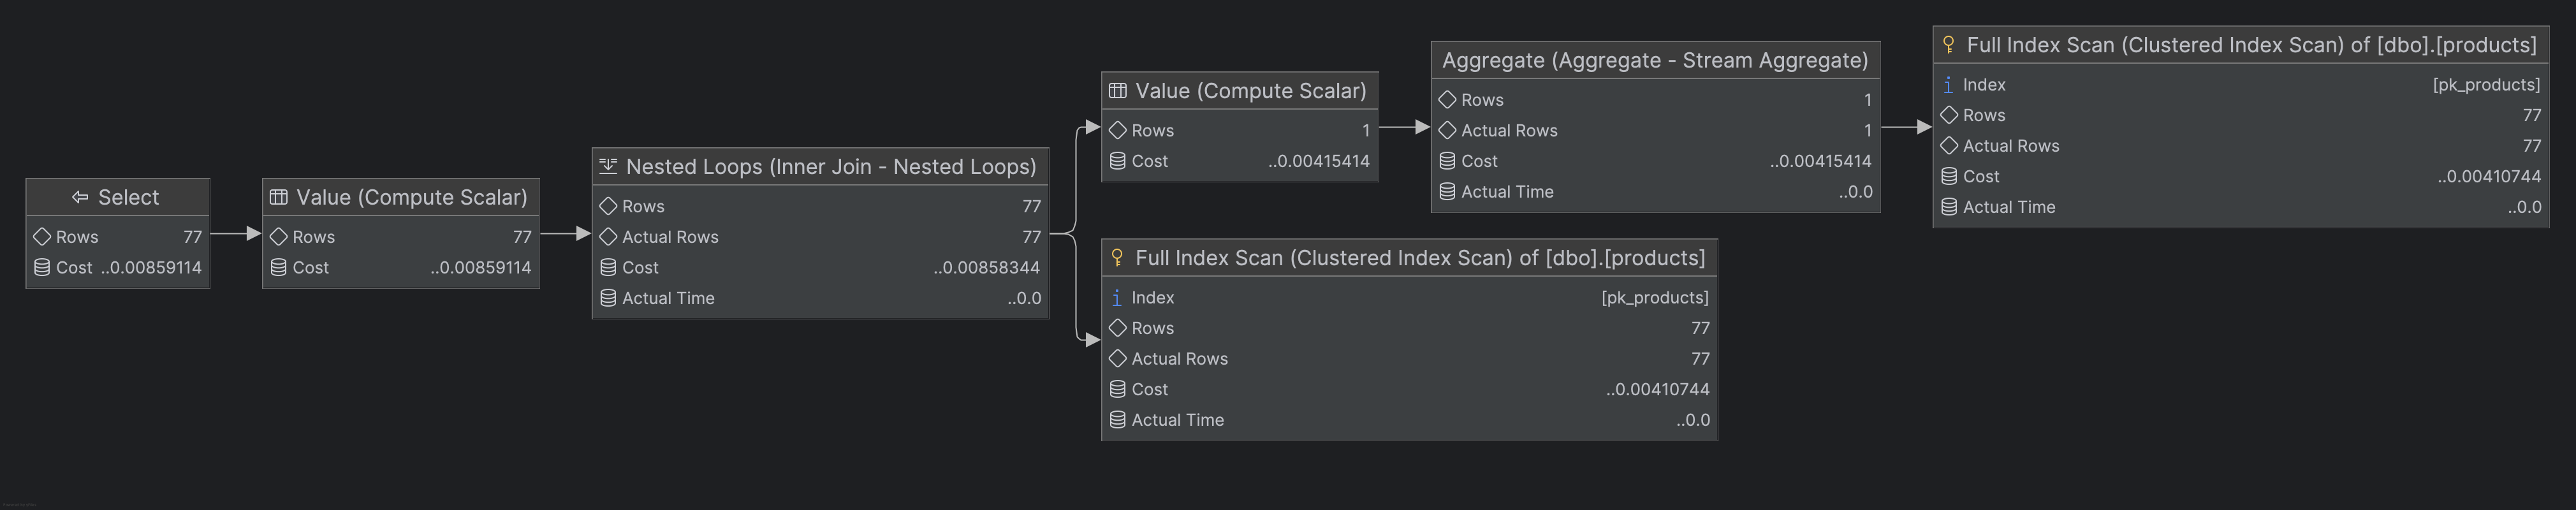
\includegraphics[width=0.8\textwidth]{../images/mssql_subquery_explain.png}
    \caption{Plan zapytania dla MSSQL - zapytanie z subquery}
    \label{fig:mssql1}
\end{figure}

\begin{figure}[H]
    \centering
    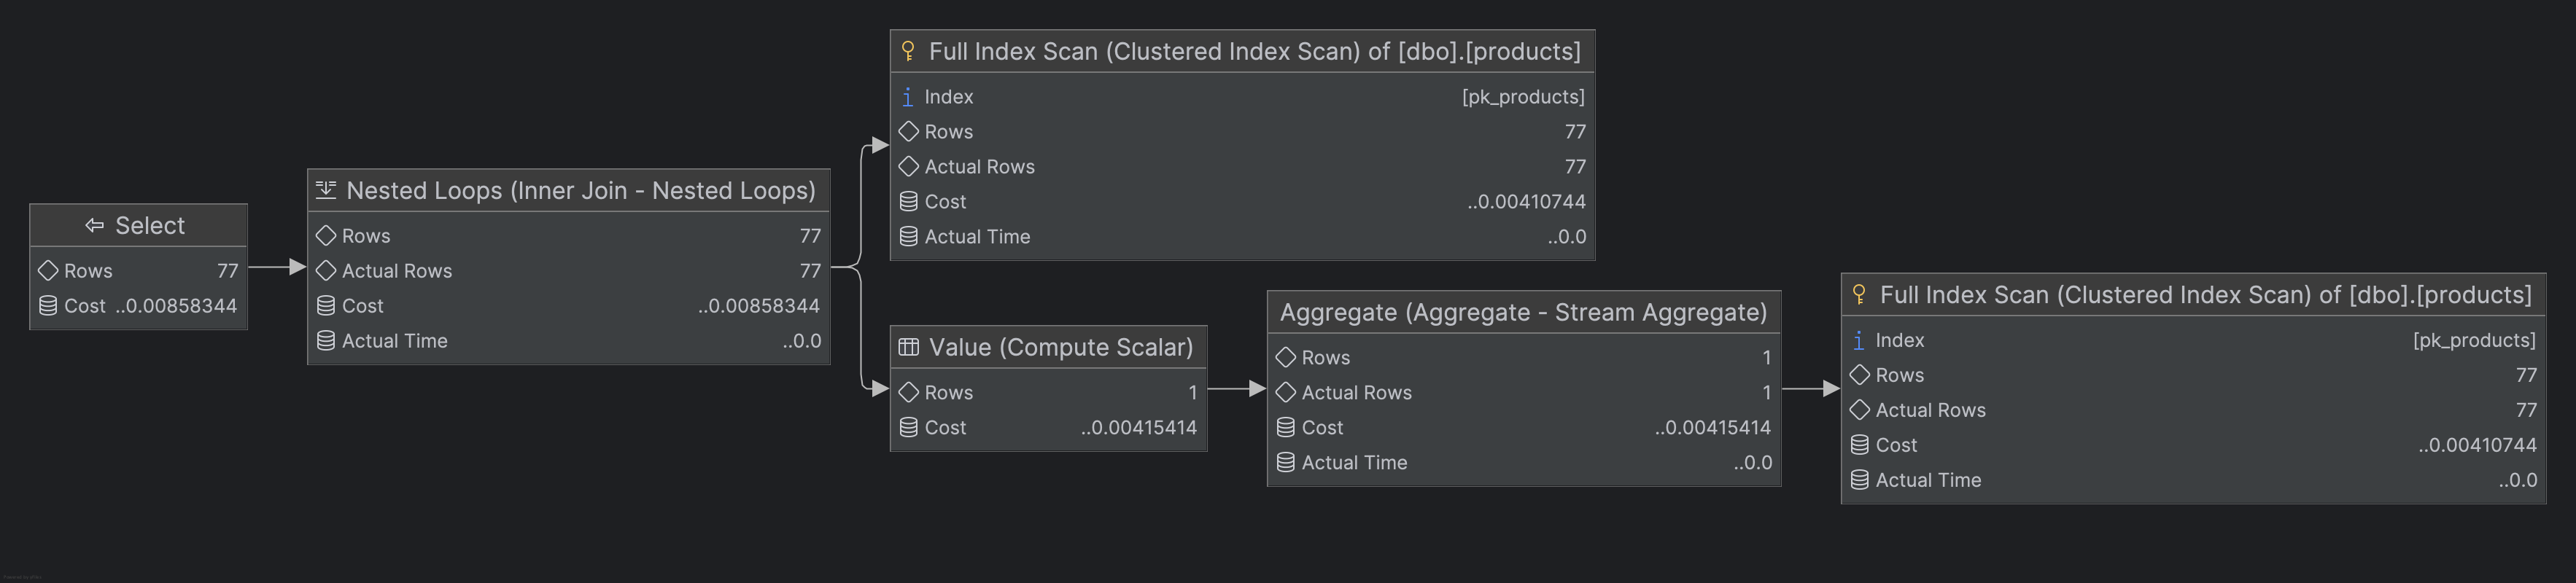
\includegraphics[width=0.8\textwidth]{../images/mssql_join_explain.png}
    \caption{Plan zapytania dla MSSQL - zapytanie z JOIN}
    \label{fig:mssql2}
\end{figure}

\begin{figure}[H]
    \centering
    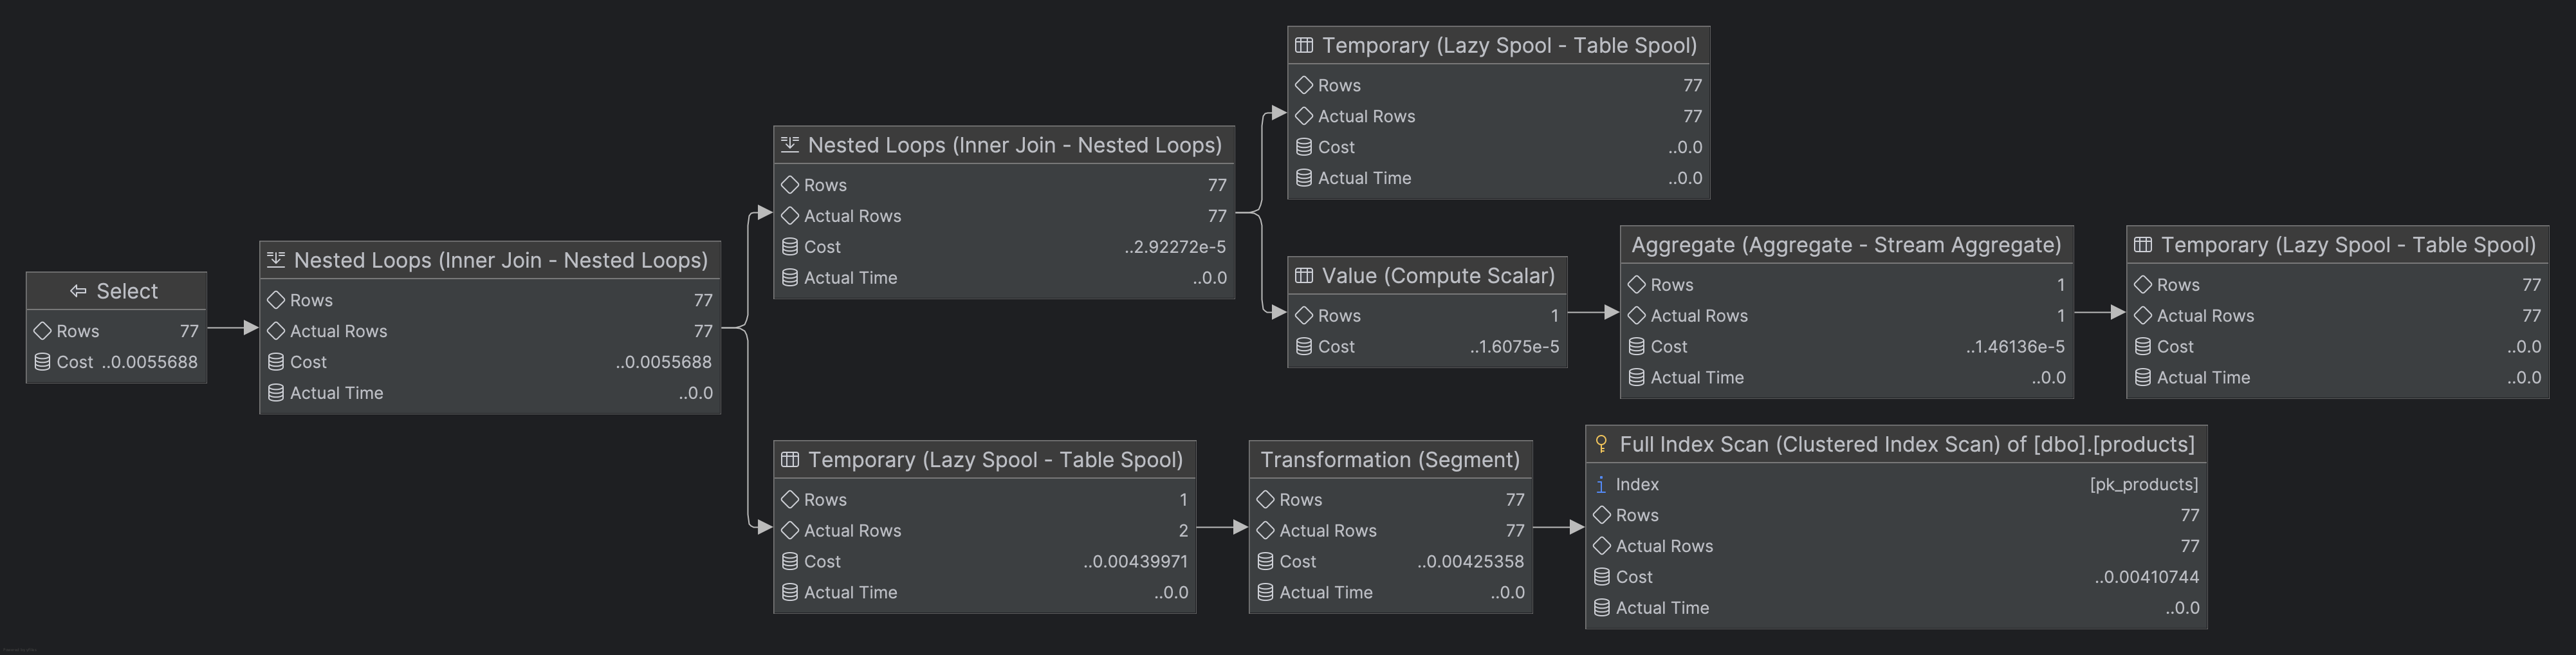
\includegraphics[width=0.8\textwidth]{../images/mssql_window_explain.png}
    \caption{Plan zapytania dla MSSQL - zapytanie z funckją okna}
    \label{fig:mssql3}
\end{figure}

\subsection*{Różnice w planach wykonania MSSQL}

Analiza wyników dla zapytań z \textbf{podzapytaniem}, \textbf{joinem} oraz \textbf{funkcją okna} w MSSQL ujawnia kilka kluczowych różnic w planach wykonania. 

1. \textbf{Podzapytanie (Subquery)}:
   W przypadku podzapytania widoczna jest dodatkowa operacja \textbf{Compute Scalar}, która oblicza wartości na podstawie warunków. Dodatkowo, zapytanie wykorzystuje \textbf{Stream Aggregate} do agregowania wyników przed dołączeniem, co wprowadza dodatkowy koszt związany z agregowaniem danych w osobnym kroku. Ponadto, zapytanie korzysta z \textbf{Clustered Index Scan}, co wskazuje na pełne skanowanie tabeli.

2. \textbf{Join}:
   Plan wykonania zapytania z \textbf{joinem} jest zbliżony do zapytania z podzapytaniem, jednak różni się brakiem osobnej agregacji. \textbf{Compute Scalar} jest nadal obecny, ale agregacja (COUNT i SUM) wykonywana jest bezpośrednio w trakcie dołączenia. Również w tym przypadku wykorzystano \textbf{Clustered Index Scan}, co sprawia, że zapytanie może być nieco bardziej wydajne niż zapytanie z podzapytaniem, ponieważ nie ma osobnego etapu agregacji.

3. \textbf{Funkcja okna (Window Function)}:
   Plan zapytania z funkcją okna jest najbardziej złożony. Zawiera dodatkowe operacje takie jak \textbf{Table Spool} i \textbf{Segment}, które pomagają w przechowywaniu wyników pośrednich. Zapytanie wykonuje \textbf{Clustered Index Scan} na tabeli, a agregacja z funkcją okna jest realizowana w obrębie samego zapytania, co może zwiększać złożoność. Jednak zastosowanie tych mechanizmów może prowadzić do bardziej efektywnego przetwarzania danych w przypadku dużych zbiorów.

\subsection*{Podsumowanie}

W przypadku MSSQL zapytania z \textbf{funkcją okna} okazują się być najbardziej złożone w wykonaniu, z dodatkowymi mechanizmami buforowania wyników i segmentowania danych. Z kolei zapytania z \textbf{podzapytaniem} i \textbf{joinem} są mniej skomplikowane, ale podzapytanie może wiązać się z wyższym kosztem z powodu osobnej agregacji. Ostateczna wydajność zależy od konkretnego przypadku i charakterystyki danych, jednak w ogólności zapytania z \textbf{funkcją okna} mogą zapewniać lepszą optymalizację przy dużych zbiorach danych.

\subsection*{PostgreSQL}

Teraz przeanalizujemy plan zapytania w systemie PostgreSQL.

\begin{figure}[H]
    \centering
    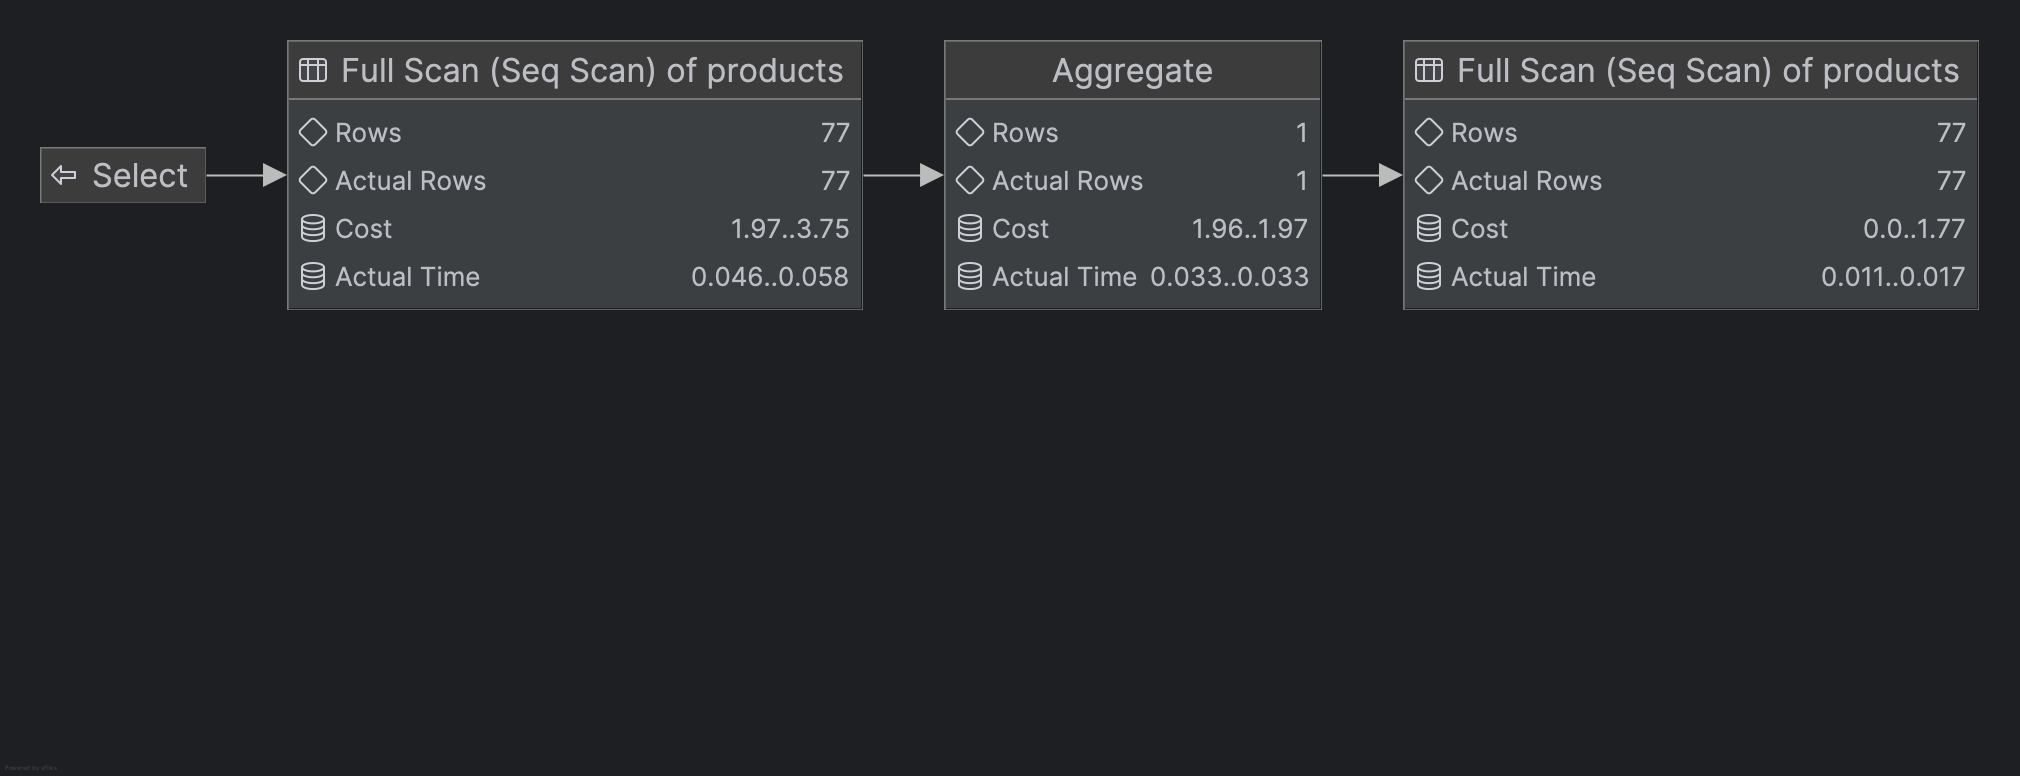
\includegraphics[width=0.8\textwidth]{../images/psql_subquery_explain.png}
    \caption{Plan zapytania dla PostgreSQL - zapytanie z subquery}
    \label{fig:postgres1}
\end{figure}

\begin{figure}[H]
    \centering
    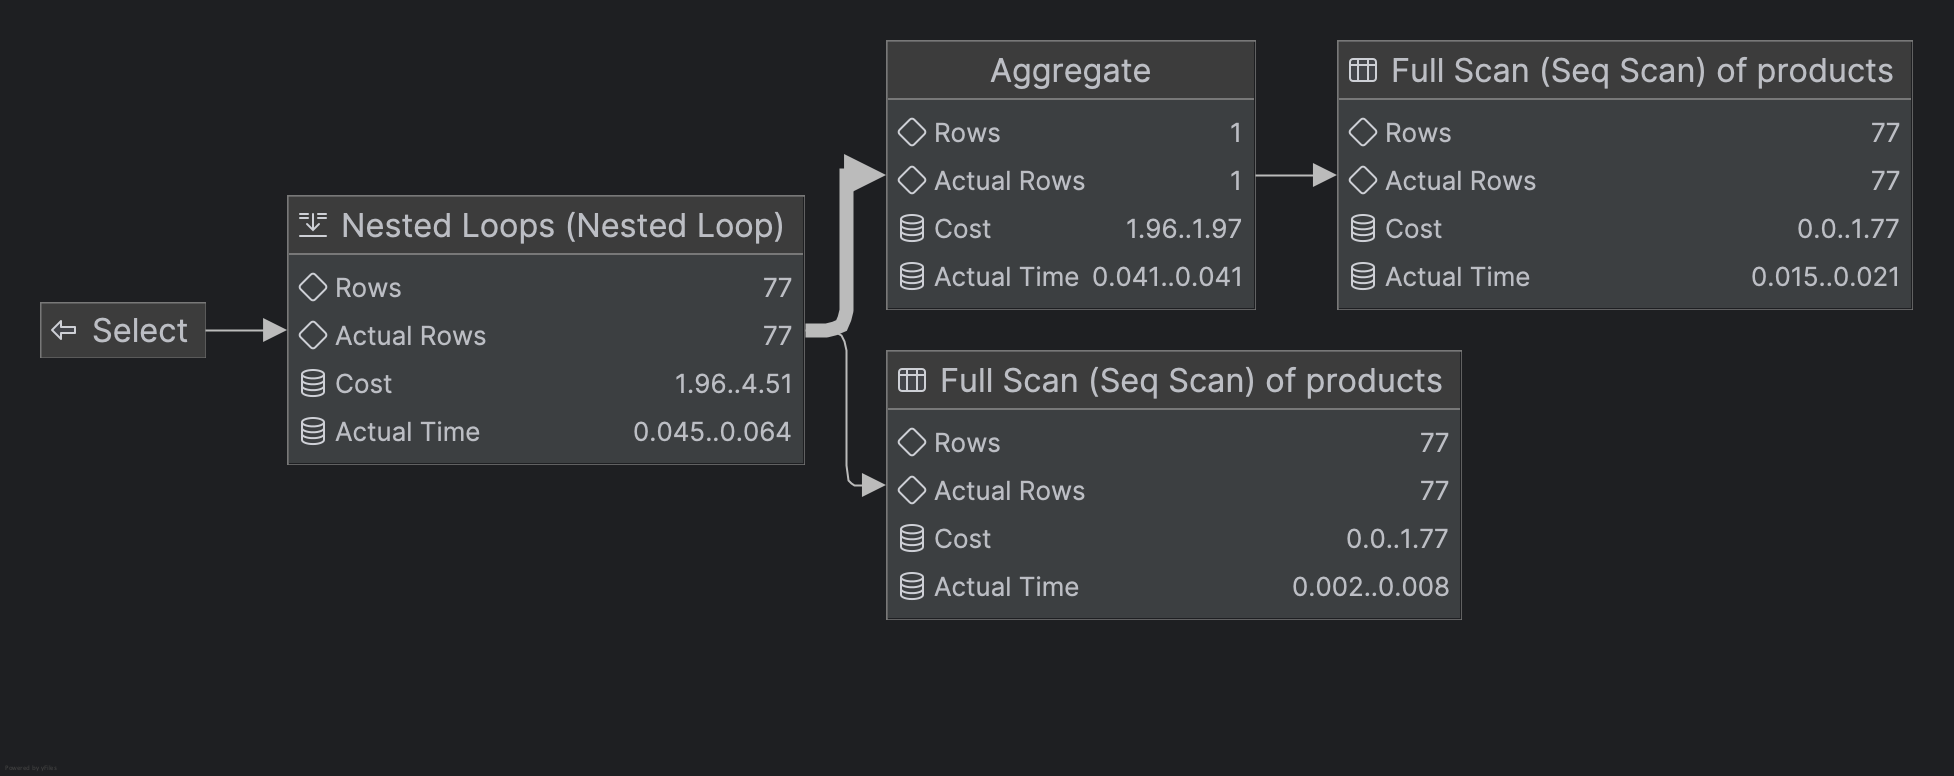
\includegraphics[width=0.8\textwidth]{../images/psql_join_explain.png}
    \caption{Plan zapytania dla PostgreSQL - zapytanie z JOIN}
    \label{fig:postgres2}
\end{figure}

\begin{figure}[H]
    \centering
    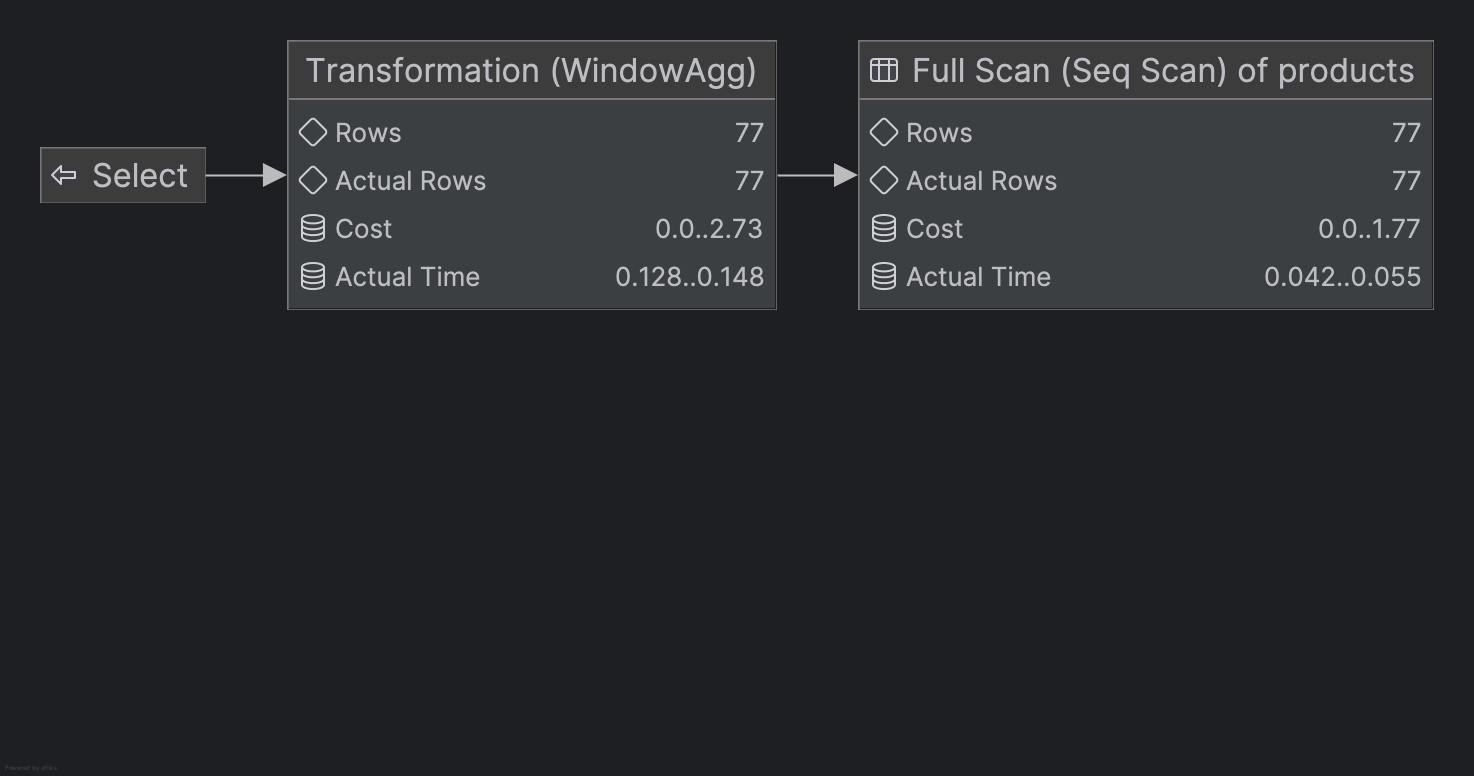
\includegraphics[width=0.8\textwidth]{../images/psql_window_explain.png}
    \caption{Plan zapytania dla PostgreSQL - zapytanie z funkcją okna}
    \label{fig:postgres3}
\end{figure}

\subsection*{Różnice w planach wykonania PSQL}

Analiza wyników \texttt{EXPLAIN ANALYZE} dla zapytań z podzapytaniem, \texttt{JOIN} oraz funkcją okna w PostgreSQL ujawnia różnice w metodzie przetwarzania danych oraz czasie wykonania:

\begin{itemize}
    \item \textbf{Subquery}: Zapytanie z podzapytaniem wykonuje pełne skanowanie tabeli \texttt{products} oraz agregację. Czas wykonania całkowity wynosi 0.383 ms, a proces agregacji jest względnie szybki (0.139..0.140 ms). Niemniej jednak, pełne skanowanie jest mniej efektywne w przypadku dużych danych.
    
    \item \textbf{Join}: W przypadku \texttt{JOIN} wykorzystano metodę \texttt{Nested Loop}, która wykonuje wielokrotne skanowanie tabeli. Czas wykonania wynosi 0.099 ms, ale przy większych zbiorach danych może być mniej skalowalne. Koszt planu jest wyższy niż w przypadku podzapytania.
    
    \item \textbf{Window}: Funkcja okna (\texttt{WindowAgg}) wykonuje się najwydajniej, chociaż koszt analizy jest wyższy niż w przypadku pozostałych zapytań. Czas wykonania wynosi 0.160 ms, co jest wynikiem przetwarzania danych w jednym przebiegu. Funkcja okna okazuje się być najbardziej wydajna w tym przypadku.
\end{itemize}

\subsection*{Podsumowanie}

Podsumowując, w analizie zapytań w PostgreSQL:
\begin{itemize}
    \item \textbf{Subquery} jest najprostsze w implementacji, ale może być mniej wydajne przy większych danych z powodu pełnego skanowania tabeli.
    \item \textbf{Join} wykorzystuje \texttt{Nested Loop}, co może być nieefektywne w przypadku dużych zbiorów danych. Mimo to, zapytanie wykonuje się szybciej niż podzapytanie.
    \item \textbf{Window} okazało się najwydajniejsze w przypadku mniejszych danych. Mimo wyższego kosztu planu, czas wykonania jest najniższy, ponieważ zapytanie przetwarza dane w jednym przebiegu, co daje lepsze rezultaty w porównaniu do \texttt{JOIN} i \texttt{Subquery}.
\end{itemize}

\subsection*{SQLite}

W przypadku SQLite, wyniki zapytania w narzędziu EXPLAIN PLAN wyglądają następująco.

\begin{figure}[H]
    \centering
    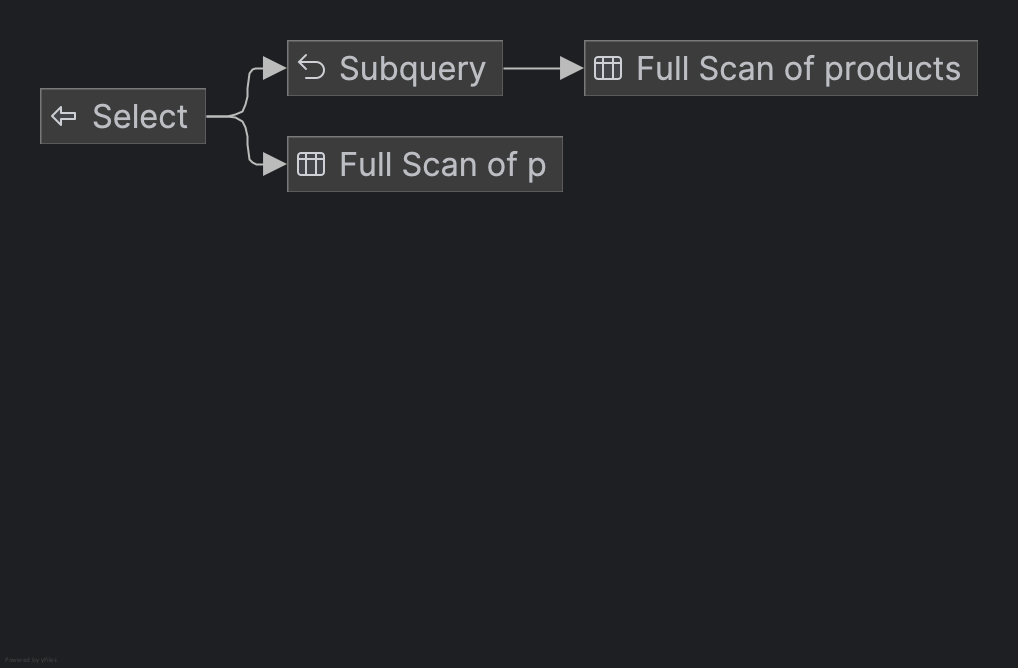
\includegraphics[width=0.8\textwidth]{../images/sqlite_subquery_explain.png}
    \caption{Plan zapytania dla SQLite - zapytanie z subquery}
    \label{fig:sqlite1}
\end{figure}

\begin{figure}[H]
    \centering
    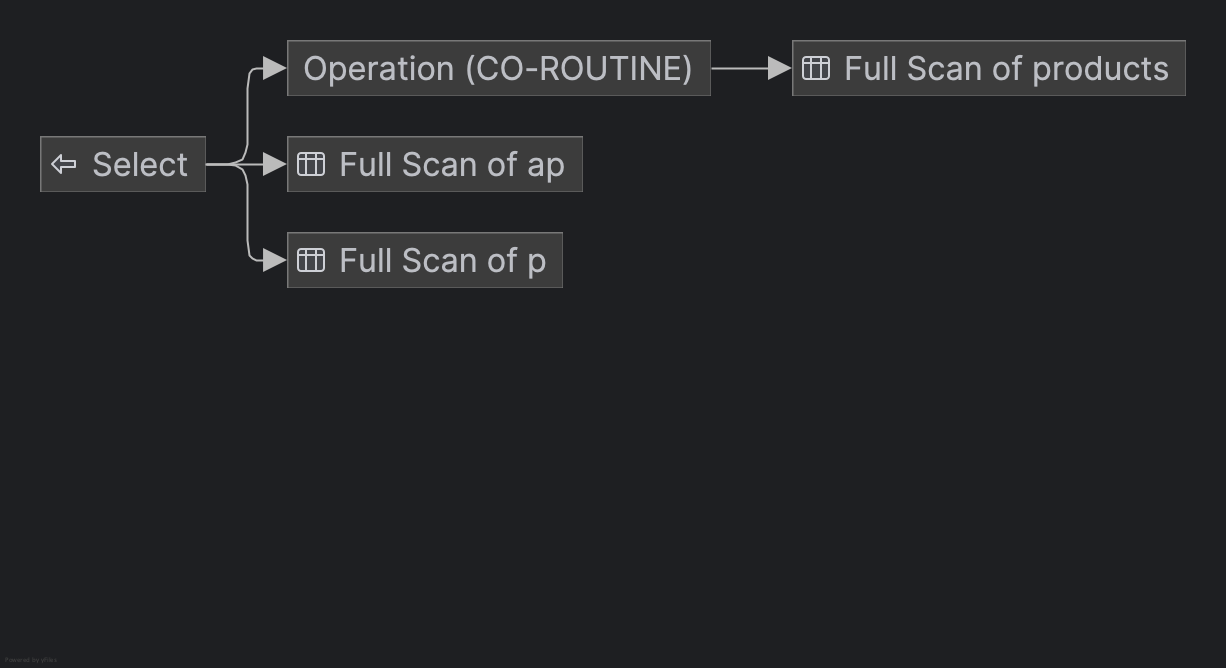
\includegraphics[width=0.8\textwidth]{../images/sqlite_join_explain.png}
    \caption{Plan zapytania dla SQLite - zapytanie z JOIN}
    \label{fig:sqlite2}
\end{figure}

\begin{figure}[H]
    \centering
    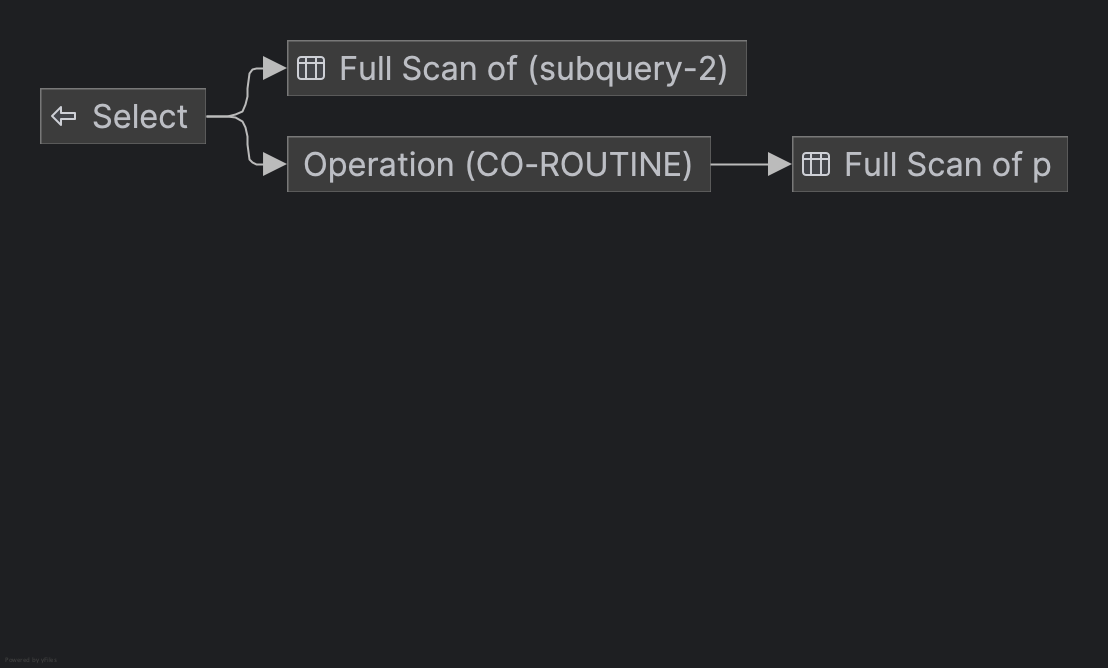
\includegraphics[width=0.8\textwidth]{../images/sqlite_window_explain.png}
    \caption{Plan zapytania dla SQLite - zapytanie z funkcją okna}
    \label{fig:sqlite3}
\end{figure}

\subsection*{Różnice w planach wykonania SQLite}

\begin{itemize}
    \item \textbf{Subquery:} Plan wykonania subquery składa się z dwóch skanów tabeli \texttt{products}. Pierwszy jest dla głównego zapytania, a drugi dla podzapytania. Jest to stosunkowo prosta operacja, choć koszt związany z oddzielnym przetwarzaniem podzapytania jest wyższy.
    \item \textbf{Join:} Plan dla zapytania z \texttt{JOIN} obejmuje cztery operacje skanowania: jedną dla tabeli \texttt{products}, jedną dla agregacji (alias \texttt{ap}), oraz dwie dla tabeli \texttt{products} (z powodu działania \texttt{JOIN}). Plan jest bardziej złożony w porównaniu do subquery.
    \item \textbf{Window Function:} Zapytanie z funkcją okna jest również złożone, ponieważ SQLite używa \texttt{CO-ROUTINE} do obliczenia agregacji w ramach funkcji okna. Skanowanie tabeli \texttt{products} i wyników funkcji okna wprowadza większą złożoność w porównaniu do prostych zapytań z \texttt{JOIN} i subquery.
\end{itemize}

\subsection*{Podsumowanie}

Porównując zapytania z \texttt{subquery}, \texttt{JOIN} oraz \texttt{Window Function} w SQLite, można zauważyć, że:
\begin{itemize}
    \item Zapytania z \texttt{subquery} są najprostsze, ponieważ wymagają tylko dwóch skanów tej samej tabeli.
    \item Zapytania z \texttt{JOIN} i \texttt{Window Function} są bardziej złożone, ponieważ wymagają więcej operacji skanowania oraz wykorzystują dodatkowe techniki, takie jak \texttt{CO-ROUTINE}.
    \item Zapytanie z funkcją okna jest najbardziej złożone, ponieważ SQLite wykonuje równoległe przetwarzanie wyników za pomocą \texttt{CO-ROUTINE} i agregacji okna.
\end{itemize}

\section*{Zadanie 4}

Poniżej znajdują się trzy różne podejścia do uzyskania rezultatu zadania: przy użyciu podzapytania, JOIN-a oraz funkcji okna.

\begin{enumerate}
    \item \textbf{Zapytanie z wykorzystaniem podzapytania}
    \begin{lstlisting}[caption={Subquery}]
        SELECT p.productid,
        p.productname,
        p.unitprice,
        avg_price
 FROM products p
          JOIN (SELECT categoryid,
                       AVG(unitprice) AS avg_price
                FROM products
                GROUP BY categoryid) avg_table
               ON p.categoryid = avg_table.categoryid
 WHERE p.unitprice > avg_table.avg_price
 ORDER BY 1;
    \end{lstlisting}

    \item \textbf{Zapytanie z wykorzystaniem JOIN-a}
    \begin{lstlisting}[caption={JOIN}]
        SELECT p.productid,
        p.productname,
        p.unitprice,
        avg_price
 FROM products p
          JOIN (SELECT categoryid,
                       AVG(unitprice) AS avg_price
                FROM products
                GROUP BY categoryid) avg_table
               ON p.categoryid = avg_table.categoryid
 WHERE p.unitprice > avg_table.avg_price
 ORDER BY 1;
    \end{lstlisting}

    \item \textbf{Zapytanie z wykorzystaniem funkcji okna}
    \begin{lstlisting}[caption={Funkcja okna}]
        WITH avg_prices AS (SELECT p.productid,
        p.productname,
        p.unitprice,
        AVG(p.unitprice) OVER (PARTITION BY p.categoryid) AS avg_price
 FROM products p)
SELECT productid,
productname,
unitprice,
avg_price
FROM avg_prices
WHERE unitprice > avg_price
ORDER BY 1;
    \end{lstlisting}
\end{enumerate}

Następnie porównałem wyniki operacji Explain Analyze dla każdego z tych zapytań dla każdej z bas danych.
W sprawozdaniu przedstawiam wyniki tylko dla PostgreSQL, w pozostalych przypadkach obserwacje dotyczace efektywnosci zapytan sa bardzo podobne.

\subsection*{PostgreSQL}
\begin{figure}[H]
    \centering
    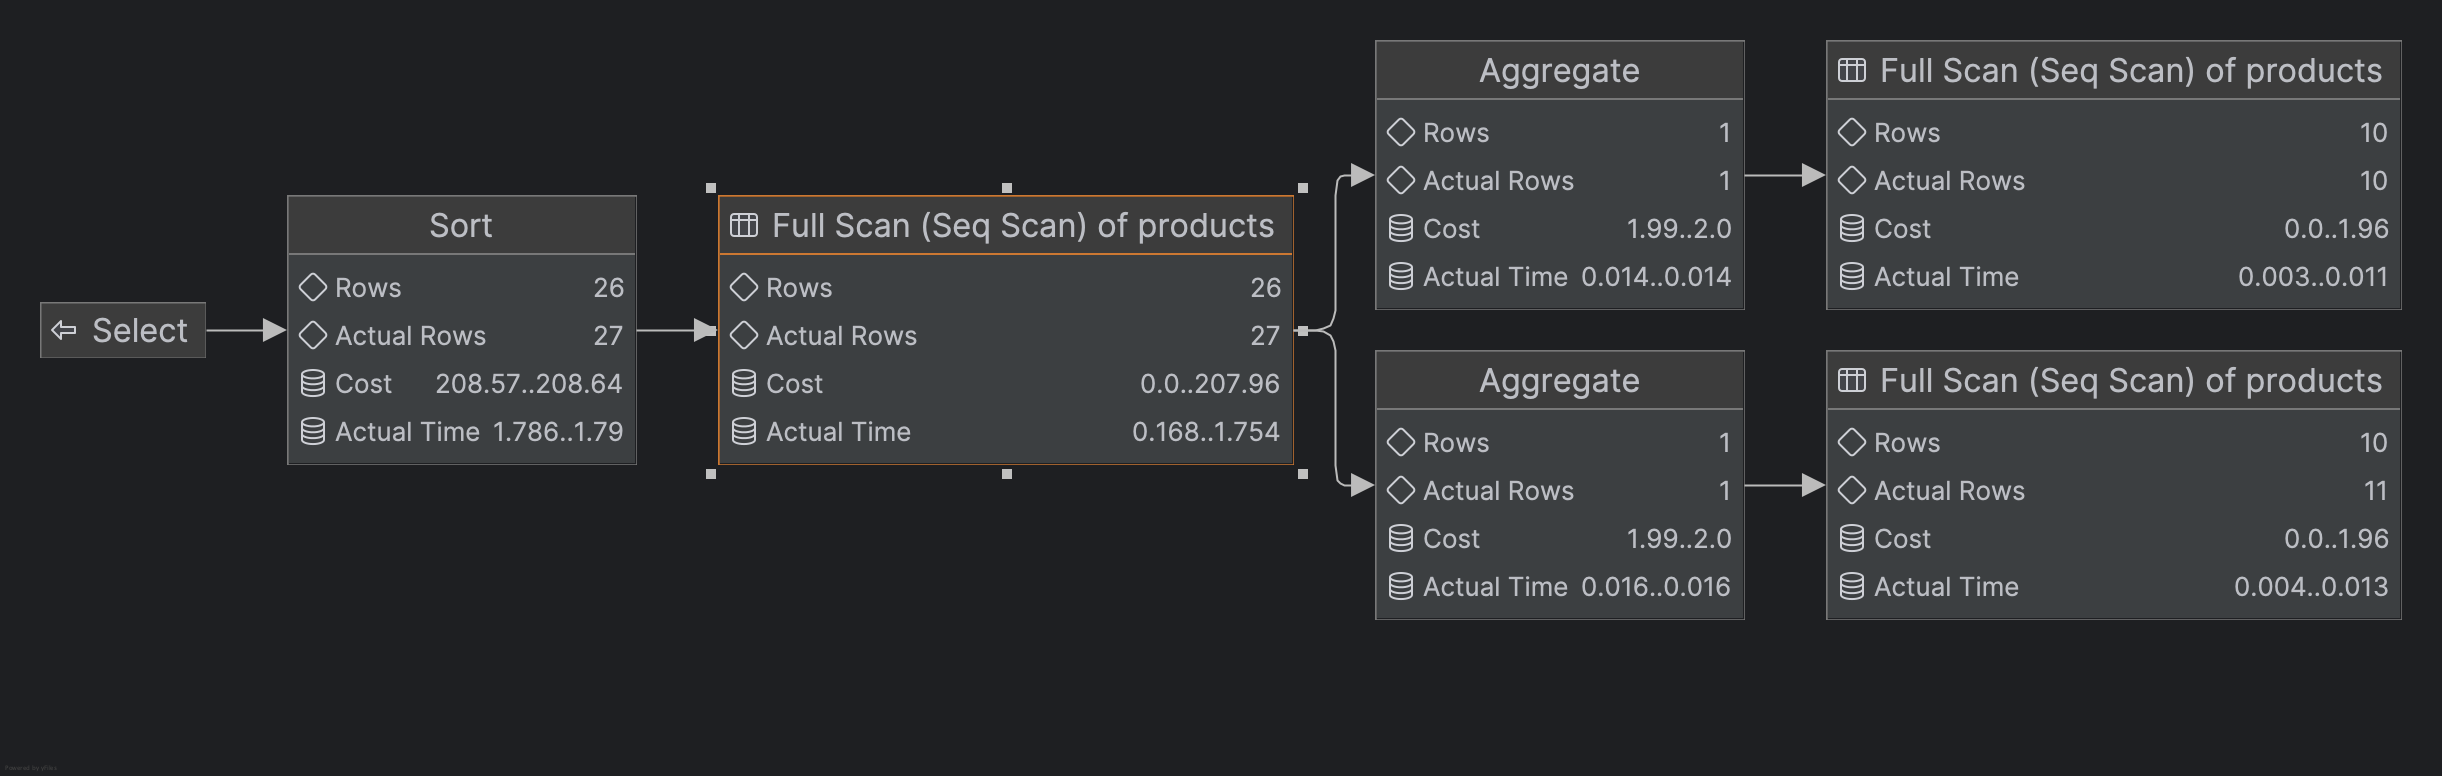
\includegraphics[width=0.8\textwidth]{../images/psql_final_subquery_explain.png}
    \caption{Plan zapytania dla PSQL - zapytanie z subquery}
\end{figure}

\begin{figure}[H]
    \centering
    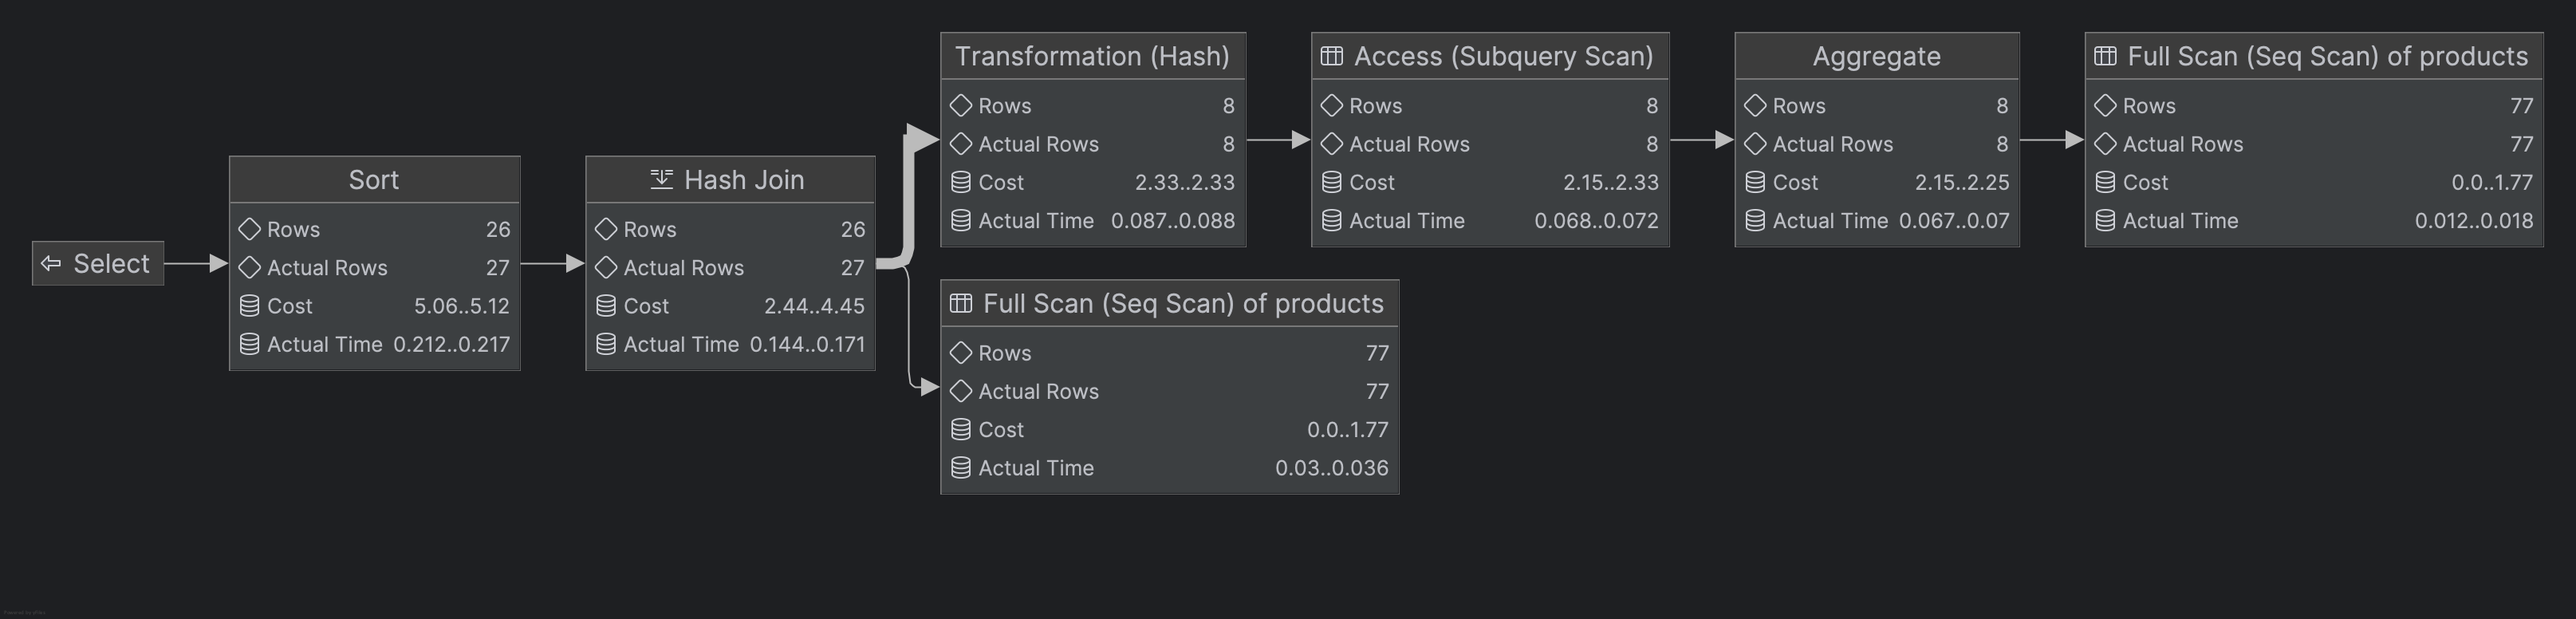
\includegraphics[width=0.8\textwidth]{../images/psql_final_join.png}
    \caption{Plan zapytania dla PSQL - zapytanie z JOIN}
\end{figure}

\begin{figure}[H]
    \centering
    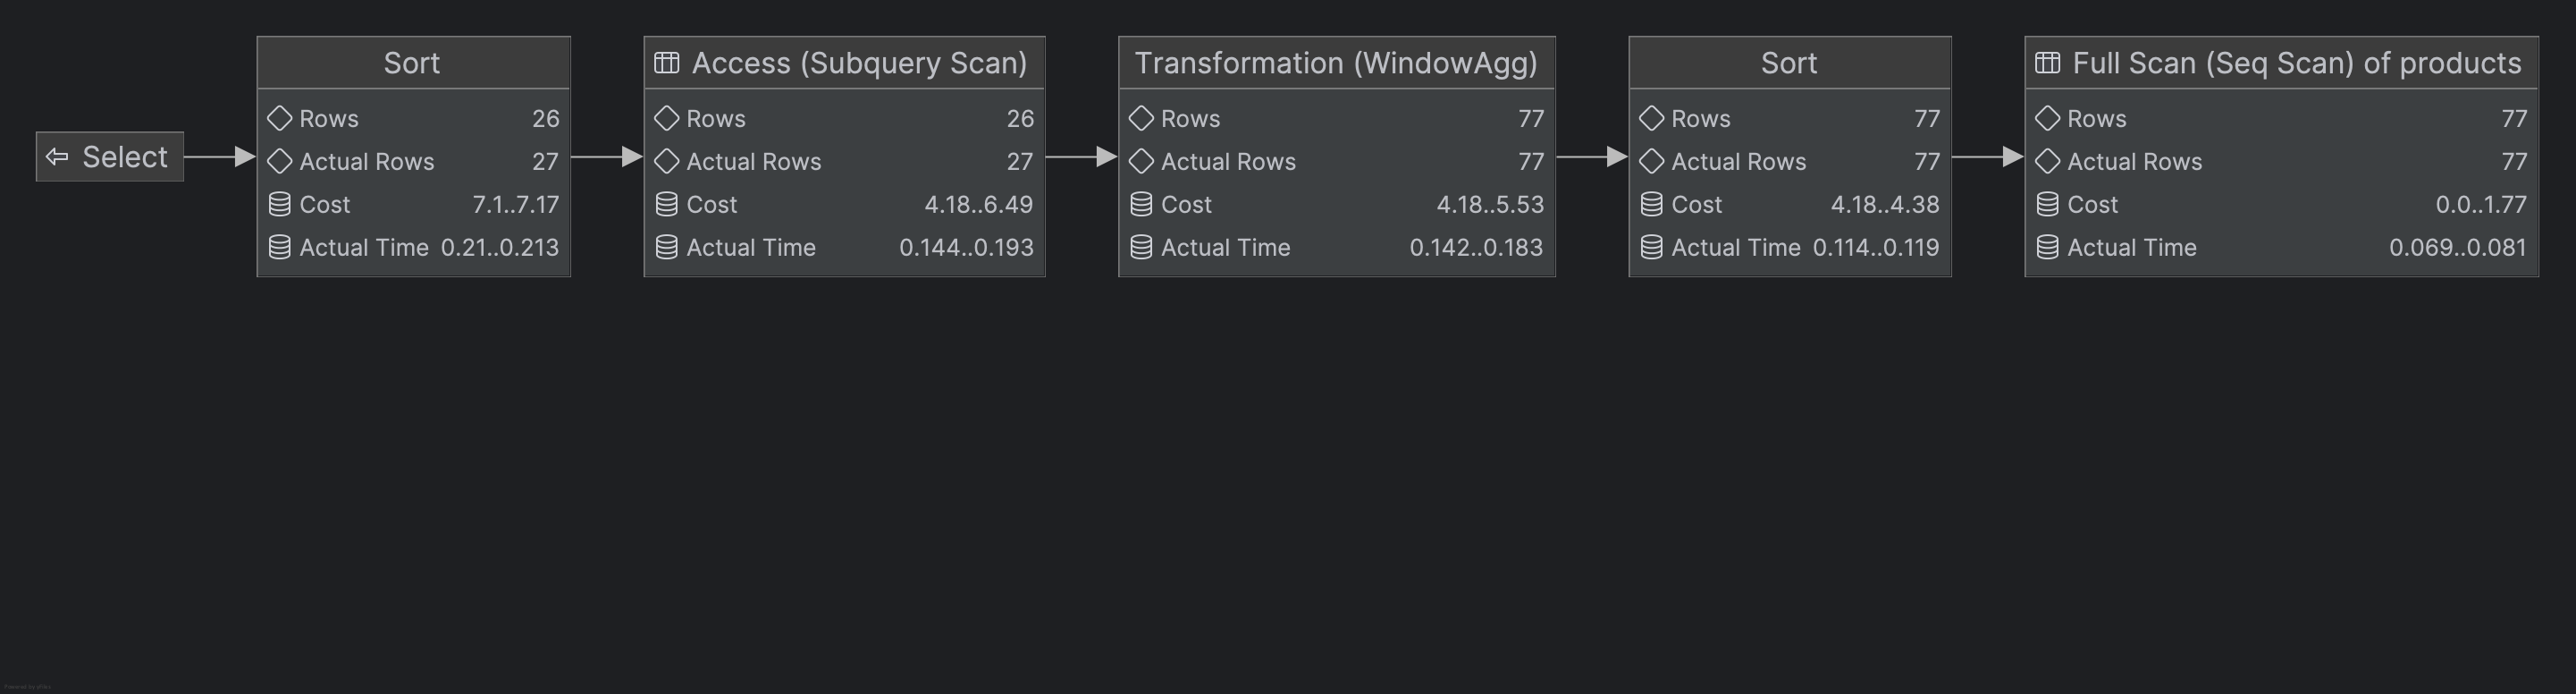
\includegraphics[width=0.8\textwidth]{../images/psql_final_window.png}
    \caption{Plan zapytania dla PSQL - zapytanie z funckją okna}
\end{figure}

\section{Analiza wydajności zapytań}
\subsection{Zapytanie z podzapytaniem (subquery)}

Dla zapytania z podzapytaniem wykonanie planu obejmuje:
\begin{itemize}
    \item Dla każdego wiersza w tabeli `products` wykonywane jest osobne podzapytanie, co prowadzi do wysokich kosztów wykonania, zwłaszcza przy dużych tabelach.
    \item Wydajność jest obniżona, ponieważ obliczenie średniej ceny dla każdej kategorii odbywa się wielokrotnie dla każdego produktu.
\end{itemize}

\subsection{Zapytanie z JOIN}

W rozwiązaniu z JOIN:
\begin{itemize}
    \item Średnia cena dla kategorii obliczana jest tylko raz w podzapytaniu, a następnie dołączana do tabeli `products`.
    \item Koszty wykonania są znacznie niższe, ponieważ średnia cena dla każdej kategorii obliczana jest raz i nie ma potrzeby wielokrotnego wykonywania podzapytań.
\end{itemize}

\subsection{Zapytanie z funkcjami okna (window functions)}

Zapytanie wykorzystujące funkcje okna (window functions):
\begin{itemize}
    \item Funkcje okna pozwalają na obliczenie średniej ceny dla każdej kategorii w jednym przejściu przez dane, bez konieczności używania podzapytań.
    \item Jest to najwydajniejsze rozwiązanie, ponieważ agregacja odbywa się w jednym kroku, a następnie używane są tylko wyniki dla każdego wiersza.
\end{itemize}

\subsection{Podsumowanie}

Najbardziej wydajne rozwiązanie to zapytanie z funkcjami okna, które oblicza średnią cenę w ramach jednej operacji. Zapytanie z JOIN również oferuje znaczną poprawę wydajności w porównaniu do zapytania z podzapytaniem, ponieważ średnia cena obliczana jest tylko raz. Zapytanie z podzapytaniem jest najwolniejsze, ponieważ wymaga obliczenia średniej ceny dla każdego produktu, co skutkuje dużym obciążeniem bazy danych przy większych ilościach obliczeń.

\begin{table}[h]
\centering
\begin{tabular}{|c|c|c|}
\hline
\textbf{Zapytanie} & \textbf{Koszt sortowania} & \textbf{Czas wykonania (ms)} \\
\hline
Podzapytanie & 208.57 & 1.540 \\
JOIN & 5.06 & 0.289 \\
Funkcje okna & 7.10 & 0.334 \\
\hline
\end{tabular}
\caption{Porównanie zapytań pod względem kosztów i czasu wykonania}
\end{table}



\end{document}
